\centerline{\bf \Large  5 класс}

\problem{\textbf{1}} Пюрвя Мучкаевич придумал систему перевода цифр в буквы и обратно, в которой каждой из десяти цифр соответствует одна уникальная буква. Он решил воспользоваться новой системой и умножил в столбик два слова УДЕ $\times$ УДЕ. Мог ли Пюрвя Мучкаевич получить в результате слово ЭРДНИЕВ? Если мог, то приведите пример таких чисел, если нет, то объясните почему.

\textbf{Решение:} Не мог получить семизначное. Заметим, что произведение двух трёхзначных чисел не может быть больше шестизначного числа, т.к. максимально можно получить 999 $\cdot$ 999 = 998001. 

\textbf{Критерии.} \\
\textit{7 баллов} $-$ Полностью верное решение\\
\textit{5 баллов} $-$ Невозможность из-за произведения, которое может быть максимально шестизначным\\
\textit{0-2 балла} $-$ Доказательство того, что максимальное произведение шестизначное\\
\textit{0 баллов} $-$ Любое решение, в котором мог\\
\textit{0 баллов} $-$ Любой ответ без объяснений\\

\problem{\textbf{2}} Решите задачу:

а) Батыр и Очир вместе решают сборник 2025 удивительных заданий Пюрви Мучкаевича за 45 дней. За сколько дней решит этот сборник один Батыр, если он за 2 дня решает столько же заданий, сколько Очир за 7 дней?

б) Составьте и решите обратную задачу по схеме: 2025; ?; 35; 2; 7.

\textbf{Решение А:} Вместе решают 2025/45=45 заданий в день. Если Батыр решает 35 заданий, а Очир 10, то условие задания выполняется. Батыр решит весь сборник за 2025/35=405/7 дня.

\textbf{Примерное условие Б:} Батыр решает сборник 2025 удивительных заданий Пюрви Мучкаевича, выполняя каждый день 35 заданий. За сколько дней решат этот сборник Батыр вместе с Очиром, если Батыр за 2 дня решает столько же заданий, сколько Очир за 7 дней?

\textbf{Решение Б:} За 2 дня Батыр решит 2$\cdot$35=70 заданий. Очир за один решает 70/7=10 заданий. Вместе решают 35+10=45 заданий в день. Вместе решат весь сборник за 2025/45=45 дней.

\textbf{Критерии.} \\
\textit{0-4 баллов} $-$ Решение пункта А\\
\textit{0-1 балла} $-$ Составление условия пункта Б \\
\textit{0-2 баллов} $-$ Решение пункта Б\\
\textit{0 баллов} $-$ Любой ответ без объяснений\\

\problem{\textbf{3}} У Данзана имеется 5 одинаковых вёдер, максимальная вместимость каждого из которых - некоторое целое число литров, и 30-литровая бочка, в которой находится целое число литров воды. Из бочки разлили всю воду по вёдрам, при этом первое ведро оказалось заполненным наполовину, второе - на треть, третье - на четверть, четвёртое - на одну пятую, пятое - на одну шестую своего объёма. Сколько литров воды было в бочке?

\textbf{Решение:} Пусть объём одного ведра равен $X$. Тогда имеем: $\dfrac{X}{2}+\dfrac{X}{3}+\dfrac{X}{4}+\dfrac{X}{5}+\dfrac{X}{6}=\dfrac{87 X}{60}=\dfrac{29 X}{20}$ будет целым только при $X$ кратном 20. Но $\mathrm{X}>20$ брать нельзя, т.к. сумма получится больше 30 литров. Значит, $X=20$. И объём воды в бочке 29 литров.

\textbf{Критерии.} \\
\textit{0-4 балла} $-$ Сложение частей и получение $\dfrac{87}{60}$\\
\textit{2 балла} $-$ Делимость на 20\\
\textit{1 балл} $-$ Можно использовать только 20\\
\textit{0-7 баллов} $-$ Перебор всех вариантов\\
\textit{0 баллов} $-$ Любой ответ без объяснений\\

\problem{\textbf{4}} Фигура \textit{Сайгак} бьёт все клетки, находящиеся от неё через клетку слева, справа, сверху или снизу, а также бьёт клетку, на которой стоит. Какое наименьшее количество \textit{Сайгаков} необходимо поставить на клетчатую доску 8 × 8 , чтобы эти фигуры били все клетки доски?

\textbf{Решение:} Раскрасим клетки доски в 4 цвета следующим образом: все клетки, куда может прийти Сайгак из, не умаляя общности, левой нижней угловой клетки, покрасим в первый цвет. Сдвигами этого множества клеток вправо, вверх и вправо вверх получаем 4 множества клеток. Рассмотрим одно из них. Чтобы все клетки были побиты, нужно как минимум 4 Сайгака, так как каждый из них бьет не более 5   клеток, и, следовательно, 3 и меньше Сайгаков бьют максимум 15 клеток. Пример расстановки 4   Сайгаков: выделим 4   непересекающихся Т-образных фигур, в каждой из которых отметим по одному Сайгаку. И так как Сайгак, стоящий на клетке из одного множества, не может дойти до клеток из трех других, получаем, что всего нужно как минимум 16 Сайгаков.

\begin{center}
    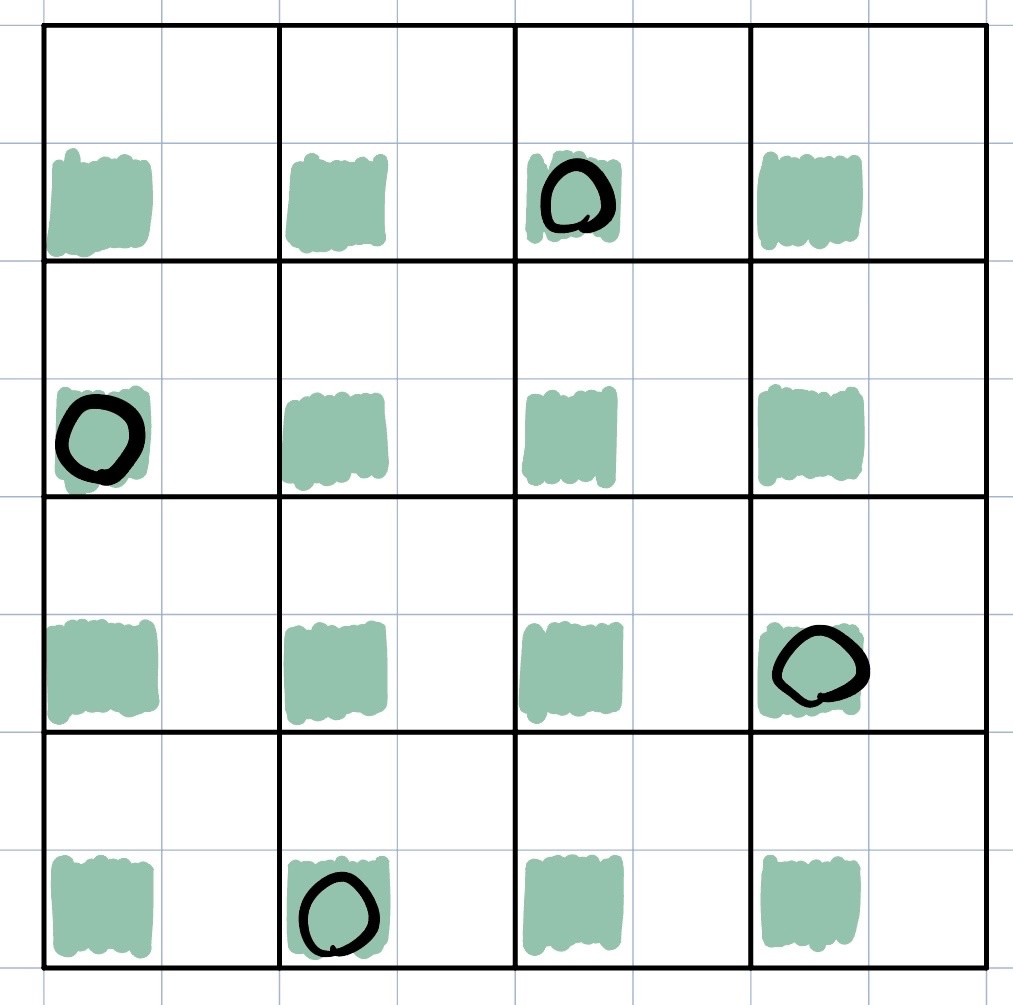
\includegraphics[width=0.3\textwidth]{Секретная информация/УДЕ 2024-2025/Регион. Решения/4.5_5.4_6.3.png}
\end{center}

\textbf{Критерии.} \\
\textit{2 балла} $-$ 16 сайгаков без объяснений\\
\textit{1 балл} $-$ Меньше 16 сайгаков без объяснений\\
\textit{0 баллов} $-$ Больше 16 сайгаков без объяснений\\
\textit{0-5 баллов} $-$ Поиск примера и оценка\\

\problem{\textbf{5}} Во дворе у Батыра есть три закрытых загона с номерами 1, 2 и 3. В одном из них 1 коричневый, 1 чёрный и 1 белый ягнёнок, в другом - 1 коричневый и 1 белый, а в третьем - 1 чёрный ягнёнок. При этом известно, что номер загона не совпадает с числом ягнят внутри загона. Как, узнав цвет только одного ягнёнка из одного загона, найти число ягнят в каждом загоне?

\textbf{Решение:} Узнаем цвет ягнёнка из 3 загона. В 3 загоне может быть 2 ягнёнка или 1, при этом сколько на самом деле ягнят определяется однозначно благодаря различным цветам (поэтому не узнаем цвет из других загонов). Если в 3 загоне 2 ягнёнка, то в 1 уже не может быть 2, а это значит, что в 1 загоне - 3 ягнёнка и во 2 загоне - 1 ягнёнок. Если же в 3 загоне 1 ягнёнок, то во 2 уже не может быть 1, а это значит, что во 2 загоне - 3 ягнёнка и в 1 загоне - 2 ягнёнка. 

\textbf{Критерии.} \\
\textit{1 балл} $-$ В первом 2 или 3, во втором 1 или 3 и в третьем 1 или 2 ягнёнка\\
\textit{0-2 балла} $-$ Однозначное определение последующих загонов, если знаешь любой один\\
\textit{0-4 балла} $-$ Подходить нужно к третьему (однозначное определение по цветам)\\
\textit{0-7 баллов} $-$ Полный перебор\\
\textit{0 баллов} $-$ Любой ответ без объяснений\\